\bookchapter{Capítulo 42: Panorama de los grandes modelos y práctica con la API}

\chapterintro{Los capítulos anteriores hablaban de «cómo colaborar con la IA»; este capítulo responde a una pregunta más básica: «¿qué IA usar y cómo?». El panorama de los grandes modelos de agosto de 2026 es riquísimo: a nivel internacional compiten los tres grandes, GPT, Claude y Gemini, mientras que en China florecen DeepSeek, Tongyi Qianwen, GLM, Kimi y Doubao. Cada modelo tiene su carácter y sus fortalezas: elegir bien te ahorra la mitad del esfuerzo; elegir mal te cuesta el doble. Este capítulo no solo te presenta estos modelos, sino que también te enseña a conectarlos a tus propias aplicaciones mediante la API y a elegir el Token Plan (plan de consumo) adecuado según tus necesidades.}

\booksection{Los grandes modelos internacionales: un terreno de tres potencias}

En el mercado internacional de grandes modelos de agosto de 2026 se ha consolidado un triángulo de potencias: OpenAI (serie GPT), Anthropic (serie Claude) y Google (serie Gemini). Cada una tiene un carácter muy marcado; vamos a conocerlas una por una.

\booksubsection{Serie GPT-5.6 de OpenAI: el todoterreno equilibrado}

OpenAI fue quien inició la ola de los grandes modelos y la serie GPT sigue siendo la más usada del mundo. La serie GPT-5.6, lanzada en julio de 2026, adopta una estrategia de tres gamas: la insignia GPT-5.6 Sol para necesidades de razonamiento avanzado, la equilibrada GPT-5.6 Terra para el desarrollo diario y la ligera GPT-5.6 Luna para escenarios de alta concurrencia y bajo costo. Los tres modelos comparten una ventana de contexto de 1,05 millones de tokens y admiten entrada de imágenes, llamadas a funciones y salida estructurada.

\begin{center}
\begin{tabularx}{\linewidth}{|X|X|X|X|X|}
\hline
\textbf{Modelo} & \textbf{Gama} & \textbf{Entrada (/millón de tokens)} & \textbf{Salida (/millón de tokens)} & \textbf{Ventana de contexto} \tabularnewline
\hline
GPT-5.6 Sol & Insignia, razonamiento & 5,00 USD ($\approx$36 CNY) & 30,00 USD ($\approx$217 CNY) & 1,05 M de tokens \tabularnewline
GPT-5.6 Terra & Equilibrada, diaria & 2,50 USD ($\approx$18 CNY) & 15,00 USD ($\approx$109 CNY) & 1,05 M de tokens \tabularnewline
GPT-5.6 Luna & Ligera, bajo costo & 1,00 USD ($\approx$7 CNY) & 6,00 USD ($\approx$44 CNY) & 1,05 M de tokens \tabularnewline
\hline
\end{tabularx}
\end{center}

\begin{center}\small\color{gray}Precios de la serie GPT-5.6 de OpenAI (agosto de 2026)\end{center}

La ventaja central de la serie GPT es su «equilibrio»: razonamiento, programación, redacción y multimodalidad, sin debilidades evidentes. Suma además el enorme ecosistema de complementos y la comunidad de desarrolladores de OpenAI, con la documentación y las cadenas de herramientas más completas. Para los casos de «no sé qué elegir», GPT es la respuesta por defecto que «no falla ni con los ojos cerrados». Sus puntos débiles: desde China se necesita red especial para acceder, su chino suena a veces «traducido» y su precio de API es de nivel medio-alto.

\textbf{Buenas noticias}\par

En agosto de 2026, OpenAI anunció que el modelo por defecto de los usuarios gratuitos pasa a ser GPT-5.6 Luna, con chat de texto ilimitado. Esto significa que puedes probar las capacidades básicas de GPT a costo cero y solo pagar cuando necesites más razonamiento o llames a la API.

\booksubsection{Serie Claude de Anthropic: la cima de la programación y el rigor}

Si GPT es el todoterreno, Claude es la «cima» del ámbito de la programación. La serie Claude de Anthropic lidera con ventaja sostenida en SWE-bench (el benchmark de ingeniería de software), con la mejor calidad de generación de código y la mayor capacidad de aterrizar proyectos a nivel de ingeniería del sector. Más destacable aún: Claude tiene la tasa de alucinaciones (probabilidad de generar información falsa) más baja de todos los modelos, de apenas un 1 \%, lo que lo hace especialmente apto para escenarios de alta precisión como la academia o lo jurídico.

El otro as en la manga de Claude es su contexto ultra largo: admite una ventana de contexto de 1 millón de tokens y puede «leer» de una sola vez cientos de páginas de contrato o un repositorio de código entero sin perder detalle. En escenarios como la refactorización de código o el análisis de documentos largos es prácticamente insustituible. Claude Code, como herramienta de programación con IA en terminal, alcanzó a mediados de 2026 unos ingresos anualizados de 2.500 millones de dólares: la mayor prueba del reconocimiento a la capacidad de programación de Claude.

\begin{center}
\begin{tabularx}{\linewidth}{|X|X|X|X|X|}
\hline
\textbf{Modelo} & \textbf{Gama} & \textbf{Entrada (/millón de tokens)} & \textbf{Salida (/millón de tokens)} & \textbf{Ventana de contexto} \tabularnewline
\hline
Claude Fable 5 & Insignia & 10,00 USD ($\approx$72 CNY) & 50,00 USD ($\approx$362 CNY) & 1 M de tokens \tabularnewline
Claude Opus 4.8 & Profesional & 5,00 USD ($\approx$36 CNY) & 25,00 USD ($\approx$181 CNY) & 1 M de tokens \tabularnewline
Claude Sonnet 5 & Económica & 2,00 USD ($\approx$14 CNY) & 10,00 USD ($\approx$72 CNY) & 1 M de tokens \tabularnewline
\hline
\end{tabularx}
\end{center}

\begin{center}\small\color{gray}Precios de la serie Claude de Anthropic (agosto de 2026; Sonnet 5 a precio promocional)\end{center}

El punto débil de Claude es el precio: la salida de Fable 5 es la más cara de todos los modelos, 50 dólares por millón de tokens. Su capacidad multimodal (comprensión de imágenes y vídeo) también es relativamente débil. Para desarrolladores individuales con presupuesto limitado, Sonnet 5 ofrece una relación calidad-precio muy destacada durante el periodo promocional.

\booksubsection{Serie Gemini de Google: el rey de la multimodalidad}

La serie Gemini de Google llegó en 2026 a la versión 3.1 Pro. Su mayor as es la multimodalidad nativa: análisis preciso de texto e imágenes, reconocimiento de tablas por OCR sin errores, extracción eficiente de fotogramas de vídeo y análisis profundo de audio y vídeo. Está profundamente integrado con el ecosistema de Google (búsqueda, correo, servicios en la nube) y destaca en la recuperación de información en tiempo real y la comprensión entre modalidades. Además admite una entrada de contexto ultra largo de 2 millones de tokens: la ventana de contexto más grande de los modelos actuales.

Gemini se posiciona como «la primera opción para razonamiento científico y escenarios multimodales». Si tu proyecto implica mucho análisis de imágenes, comprensión de vídeo o cálculo científico, Gemini casi no tiene rival. Pero en la generación de código de texto puro queda algo por detrás de Claude, y su chino tampoco resulta tan natural como el de los modelos chinos.

\begin{center}
\begin{tabularx}{\linewidth}{|X|X|X|X|}
\hline
\textbf{Aspecto} & \textbf{GPT-5.6} & \textbf{Claude Fable 5} & \textbf{Gemini 3.1 Pro} \tabularnewline
\hline
Puntuación global & 94.8 & 95.0 & 92.1 \tabularnewline
Programación (SWE-bench) & 74.9\% & 64.3\% (Pro) & Media \tabularnewline
Ventana de contexto & 1,05 M de tokens & 1 M de tokens & 2 M de tokens \tabularnewline
Capacidad multimodal & Equilibrada & Débil & La más fuerte \tabularnewline
Tasa de alucinaciones & Baja & La más baja ($\approx$1 \%) & Baja \tabularnewline
Disponibilidad desde China & Requiere red especial & Requiere red especial & Requiere red especial \tabularnewline
Ecosistema de API & El más completo & En crecimiento & Ligado al ecosistema de Google \tabularnewline
\hline
\end{tabularx}
\end{center}

\begin{center}\small\color{gray}Comparativa de los tres grandes modelos internacionales (agosto de 2026)\end{center}

\begin{tcbwarn}{Ojo: el obstáculo real para usarlos desde China}
Para los desarrolladores en China, el obstáculo principal de GPT, Claude y Gemini es el acceso por red. Aunque se pueden usar de forma indirecta mediante proxies de Azure, plataformas agregadoras de API y otros medios, la estabilidad y el cumplimiento normativo deben evaluarse por tu cuenta. Si tu proyecto tiene requisitos estrictos de seguridad de datos, conviene priorizar los modelos chinos.

\end{tcbwarn}

\booksection{Los grandes modelos chinos: cien flores en flor}

En 2026 los grandes modelos chinos han pasado de «perseguidores» a «corredores en paralelo», e incluso a «líderes» en algunos campos. A diferencia de la polémica de 2023 sobre los «envoltorios», los modelos insignia chinos de 2026 ya están a la altura de los modelos internacionales de primera línea en razonamiento lógico, generación de código y comprensión del chino, con una brecha reducida a menos del 5 \%. Más importante aún: los modelos chinos tienen ventajas insustituibles en escenarios en chino, costos y despliegue conforme a la normativa.

\booksubsection{DeepSeek V4: el rey de la relación calidad-precio}

DeepSeek es un fenómeno entre los grandes modelos chinos. A principios de 2025, DeepSeek-V3 sacudió el mercado con su posicionamiento de «una décima parte del precio de GPT y la misma capacidad», y el sector la llamó «la línea de matanza de los grandes modelos de IA de propósito general»: no hay nada más barato que funcione tan bien, ni nada más caro que dé tanta potencia y cantidad. En agosto de 2026 se lanzó la versión oficial de DeepSeek V4-Pro: arquitectura MoE de 1,6 billones de parámetros con unos 49B activados, contexto sin pérdida de 1 millón de tokens y una relación calidad-precio en código considerada ampliamente como la mejor del mundo.

DeepSeek V4 dio un gran salto en capacidades de agente: el benchmark DeepSWE pasó de 12,8 a 62,7 (+390 \%) y NL2Repo subió de 38,5 a 61,5. Su API añadió soporte de doble protocolo (Responses API y Anthropic API) y ya es compatible con herramientas de programación populares como Codex y Claude Code. Esto significa que puedes sustituir la API de Claude por la de DeepSeek dentro de Claude Code: el costo baja varias veces y la experiencia es casi idéntica.

\begin{center}
\begin{tabularx}{\linewidth}{|X|X|X|X|X|}
\hline
\textbf{Modelo} & \textbf{Gama} & \textbf{Entrada (/millón de tokens)} & \textbf{Salida (/millón de tokens)} & \textbf{Ventana de contexto} \tabularnewline
\hline
DeepSeek V4 Pro & Insignia, razonamiento & 3 CNY ($\approx$0,43 USD) & 6 CNY ($\approx$0,87 USD) & 1 M de tokens \tabularnewline
DeepSeek V4 Flash & Ligera, rápida & 1 CNY ($\approx$0,14 USD) & 2 CNY ($\approx$0,28 USD) & 1 M de tokens \tabularnewline
\hline
\end{tabularx}
\end{center}

\begin{center}\small\color{gray}Precios de la serie DeepSeek V4 (agosto de 2026, precios promocionales)\end{center}

Comparación de precios: con el mismo 1 millón de tokens de entrada + 1 millón de salida, DeepSeek V4 Flash cuesta unos 0,42 dólares, GPT-5.6 Sol unos 35 dólares y Claude Fable 5 unos 60 dólares. Una brecha de hasta 80-140 veces.

\textbf{Aviso para evitar sorpresas: DeepSeek va a subir precios}\par

DeepSeek anunció oficialmente el 6 de agosto de 2026 que «planea subir de forma sustancial el precio de su API en breve», así que los precios promocionales pueden no durar mucho. Algunos medios rumoraron que el aumento podría llegar a 30 veces, y hasta el 14 de agosto la empresa no había publicado el plan de precios definitivo. Además, la versión oficial de DeepSeek V4 introduce un esquema de precios por horas valle y pico: en horas pico, la llamada cuesta el doble. Consulta los anuncios oficiales para conocer los precios más recientes.

\booksubsection{Tongyi Qianwen Qwen3.7 Max: la opción empresarial de Alibaba Cloud}

La serie Tongyi Qianwen (Qwen) de Alibaba Cloud se apoya en su ecosistema y tiene ventajas naturales en el despliegue empresarial. El Qwen3.7 Max de julio de 2026 es la insignia actual: un modelo denso de 235B de parámetros, con contexto nativo de 256K ampliable a 1M. Las ventajas centrales de Qwen: un ecosistema de código abierto maduro (toda la serie, de 7B a 235B, es abierta), una comprensión precisa de los escenarios en chino y una integración profunda con la infraestructura de Alibaba Cloud.

\begin{center}
\begin{tabularx}{\linewidth}{|X|X|X|}
\hline
\textbf{Modelo} & \textbf{Precio de salida (/millón de tokens)} & \textbf{Casos de uso} \tabularnewline
\hline
qwen-turbo & 0,6 CNY & Preguntas y respuestas simples, clasificación de texto, alta concurrencia \tabularnewline
qwen-long & 2,0 CNY & Procesamiento de contexto ultra largo de 10M \tabularnewline
qwen3.7-flash & 7,2 CNY & Conversación general, generación de contenido \tabularnewline
qwen3.7-plus & 12,0 CNY & Multimodal (imágenes + vídeo), creación en chino \tabularnewline
qwen3.7-max & 36,0 CNY & Capacidad insignia en chino, tareas complejas \tabularnewline
\hline
\end{tabularx}
\end{center}

\begin{center}\small\color{gray}Precios escalonados de la serie Qwen de Tongyi Qianwen (agosto de 2026)\end{center}

Qwen fija sus precios por tramos: desde el ultrabarato qwen-turbo (salida a 0,6 CNY por millón de tokens) hasta la insignia qwen3.7-max (salida a 36 CNY por millón de tokens), cubriendo todo el abanico, de las preguntas ligeras al razonamiento complejo. Para las empresas que ya usan Alibaba Cloud, Qwen es la opción de integración más cómoda.

\booksubsection{GLM-5.1 de Zhipu: número 1 chino en SWE-bench}

La serie GLM de Zhipu AI brilló en 2026. GLM-5.1 logró el primer puesto entre los modelos chinos en SWE-bench: arquitectura híbrida MoE-densa de 744B con soporte de 1 millón de tokens de contexto. Se caracteriza por una comprensión semántica del chino muy precisa y por admitir el despliegue privado conforme a la normativa china, algo crucial para escenarios como las finanzas y la administración pública, con requisitos estrictos de seguridad de datos. GLM-5.1 se ofrece a 6 CNY de entrada y 24 CNY de salida por millón de tokens, un nivel intermedio entre los modelos chinos.

\booksubsection{Kimi K3: el rey del texto ultra largo}

La serie Kimi de Moonshot AI es famosa por procesar textos ultra largos. Kimi K3, lanzado en julio de 2026, alcanza los 2,8 billones de parámetros y entra en la élite mundial en varias evaluaciones de tareas complejas. El terreno natural de Kimi es el análisis de bases de código grandes y la generación aumentada por recuperación de documentos largos: puede procesar el texto de un libro entero o el código de un proyecto completo, y destaca en las tareas de búsqueda de «agujas en un pajar». Su precio es relativamente alto (salida de unos 12-20 CNY por millón de tokens), pero su relación calidad-precio en textos largos no tiene competencia.

\booksubsection{Doubao: el todoterreno de ByteDance}

La serie Doubao de ByteDance se mantuvo estable en 2026. Doubao Seed 2.1 Pro es el modelo insignia de Volcengine, con contexto de 256K, un rendimiento general estable en pruebas reales y una experiencia destacada en chino. Las ventajas de Doubao: regala una gran cantidad de tokens gratis al registrarte, se integra muy bien en el ecosistema de Volcengine y su precio está entre los más bajos de China. Para principiantes que quieran probar rápido la programación con IA, Doubao es una puerta de entrada sin barreras.

\begin{center}
\begin{tabularx}{\linewidth}{|X|X|X|X|X|X|}
\hline
\textbf{Aspecto} & \textbf{DeepSeek V4} & \textbf{Qwen3.7 Max} & \textbf{GLM-5.1} & \textbf{Kimi K3} & \textbf{Doubao 2.1 Pro} \tabularnewline
\hline
Puntuación global & 87.5 & 89.7 & 90.5 & 88+ & 85+ \tabularnewline
Programación & Altísima & Fuerte & N.º 1 chino en SWE & Fuerte & Media-alta \tabularnewline
Comprensión del chino & Excelente & Excelente & Precisa & Excelente & Excelente \tabularnewline
Ventana de contexto & 1 M & 256K-1M & 1 M & Ultra larga & 256K \tabularnewline
Precio de salida (CNY/M) & 6 & 36 & 24 & 12-20 & 30 \tabularnewline
Código abierto & Licencia MIT & Toda la serie abierta & Parcialmente abierto & Cerrado & Cerrado \tabularnewline
Despliegue privado & Sí & Sí & Sí & No & No \tabularnewline
\hline
\end{tabularx}
\end{center}

\begin{center}\small\color{gray}Comparativa de los cinco grandes modelos chinos (agosto de 2026)\end{center}

Una tendencia importante: ya desapareció la sensación de «generación de diferencia» entre los modelos chinos y GPT/Claude. En razonamiento lógico y competiciones matemáticas, la diferencia entre los insignia chinos y GPT-5 es de apenas un dígito. En pensamiento arquitectónico sistémico y razonamiento de ingeniería compleja, Claude sigue adelante: propone soluciones de arquitectura con más «chispa», mientras que los modelos chinos a veces resultan «doctrinarios». Pero en escenarios en chino, control de costos y despliegue conforme a la normativa, los modelos chinos tienen una ventaja arrolladora.

\begin{center}
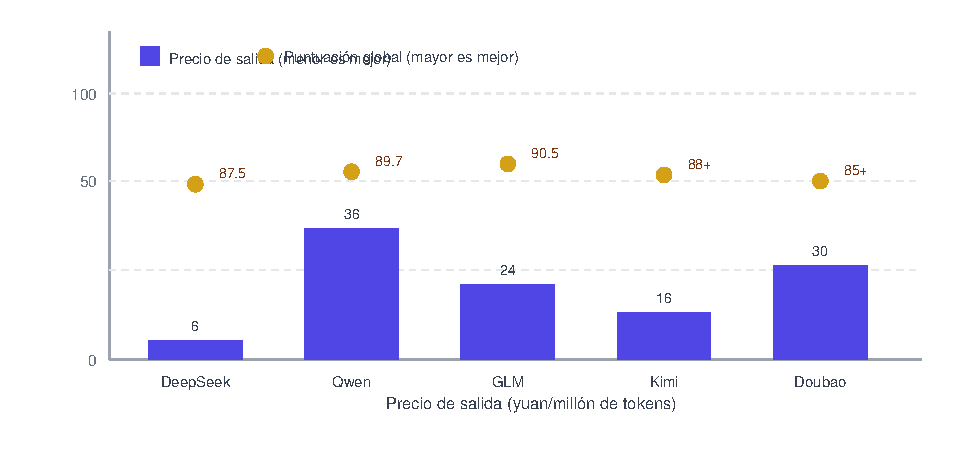
\includegraphics[width=0.92\linewidth]{figures/fig-di-si-shi-er-zhang-1}
\\[2pt]\small Figura 4: comparación de precio y rendimiento de los cinco modelos (mejor cuanto más bajo el precio y más alta la puntuación)
\end{center}

\booksection{Marco de decisión para elegir modelo}

Ya que conoces las particularidades de cada modelo, ¿cómo elegir uno para tu proyecto? Aquí tienes el «método de decisión de cuatro preguntas»: responde cuatro preguntas y darás con el modelo que mejor te conviene.

¿Tu proyecto se despliega en China o a nivel internacional?

En China elige modelos nacionales

|

Internacional modelos extranjeros como opción

¿La tarea principal es programar u otra cosa?

Programación Claude o DeepSeek

|

Otra cosa sigue evaluando

¿Necesitas un contexto muy largo (>500 000 tokens)?

Sí Gemini o Kimi

|

No hace falta sigue evaluando

¿Presupuesto ajustado?

Ajustado DeepSeek o Qwen-turbo

|

No tanto GPT-5.6 o Claude

\begin{center}\small\color{gray}Figura 5: método de decisión de cuatro preguntas para elegir un gran modelo\end{center}

\begin{tcbinfo}{Consejo: estrategia de combinación}
Este método de decisión no es un dogma: muchos escenarios requieren combinar varios modelos. Una estrategia común: DeepSeek o Qwen para el desarrollo diario (baratos y buenos en chino), Claude para el diseño de arquitecturas clave (razonamiento fuerte y pocas alucinaciones) y Gemini para el análisis multimodal (procesamiento de imágenes y vídeo). Cambia de modelo según lo que necesites, en vez de «usar uno hasta el final de los tiempos».

\end{tcbinfo}

\booksection{Primeros pasos con la API: integrar un gran modelo desde cero}

Muchos tutoriales de programación con IA solo enseñan a usar la interfaz de chat, pero la verdadera «programación con IA» —hacer que tu aplicación llame a un gran modelo— pasa por la API. La API (Application Programming Interface, interfaz de programación de aplicaciones) es el protocolo de comunicación entre programas. Con la API, tu código puede invocar la capacidad de un gran modelo igual que llama a una función.

\booksubsection{Qué es un token}

Antes de entender la API hay que comprender el concepto de «token». El token es la unidad básica de facturación de los grandes modelos; puedes verlo como la «unidad de lectura y escritura de la IA». Un token equivale aproximadamente a 0,75 palabras en inglés (4 caracteres) y a entre 0,5 y 1 carácter chino. Un texto chino de 1000 caracteres consume unos 1500-2000 tokens.

Un token no es una palabra ni un carácter. Los grandes modelos usan un tokenizador especializado para dividir el texto en tokens. La misma palabra puede ocupar un número distinto de tokens en cada modelo: por ejemplo, «inteligencia artificial» puede ser 3 tokens en GPT y 2 en DeepSeek. La API de la mayoría de los modelos devuelve el número real de tokens consumidos, y puedes consultarlo en la respuesta.

\begin{tcbinfo}{Estimación rápida del costo en tokens}
1 millón de caracteres chinos equivalen a unos 1,5 millones de tokens. Procesar 1 millón de caracteres de entrada + 1 millón de salida con DeepSeek V4 Flash cuesta unos 0,42 dólares (unos 3 CNY); con Claude Fable 5, la misma cantidad cuesta unos 60 dólares (unos 434 CNY). Por eso la elección del modelo afecta directamente al costo de tu proyecto.

\end{tcbinfo}

\booksubsection{Obtener una API Key}

El primer paso para usar la API de un gran modelo es obtener una API Key, una clave usada para autenticarte. Cada proveedor de modelos tiene su propia plataforma de API, donde debes registrarte y crear la API Key. Estas son las plataformas de API de los modelos principales, con su proceso de obtención:

\begin{center}
\begin{tabularx}{\linewidth}{|X|X|X|X|}
\hline
\textbf{Modelo} & \textbf{Plataforma de API} & \textbf{Proceso de obtención} & \textbf{Cuota gratuita} \tabularnewline
\hline
DeepSeek & platform.deepseek.com & Registro verificación de identidad crear API Key & Cuota de regalo para nuevos usuarios \tabularnewline
Tongyi Qianwen & bailian.aliyun.com (plataforma Bailian) & Iniciar sesión con cuenta de Alibaba Cloud activar el servicio crear la Key & Prueba gratuita para nuevos usuarios \tabularnewline
Zhipu GLM & open.bigmodel.cn & Registro verificación de identidad crear API Key & Cuota de regalo para nuevos usuarios \tabularnewline
Kimi & platform.moonshot.cn & Registro verificación de identidad crear API Key & Cuota gratuita limitada \tabularnewline
Doubao & volcengine.com (Volcengine) & Registro activar Ark crear API Key & Regala muchos tokens al registrarte \tabularnewline
OpenAI GPT & platform.openai.com & Registro vincular tarjeta de crédito crear API Key & Sin cuota gratuita (de pago) \tabularnewline
Anthropic Claude & console.anthropic.com & Registro vincular tarjeta crear API Key & Cuota pequeña para nuevos usuarios \tabularnewline
\hline
\end{tabularx}
\end{center}

\begin{center}\small\color{gray}Plataformas de API de los modelos principales y cómo obtener la Key (agosto de 2026)\end{center}

\textbf{Aviso de seguridad: la API Key es como la contraseña de tu monedero}\par

La API Key equivale a la contraseña de tu monedero: cualquiera que la consiga puede usar tu cuota para llamar al modelo. Por eso: nunca escribas la API Key en el código (gestiónala con variables de entorno); nunca subas a un repositorio Git público código que contenga la Key; nunca compartas en redes sociales capturas donde aparezca. Si la Key se filtra, bórrala de inmediato en la plataforma y crea una nueva.

\booksubsection{Tu primera llamada a la API}

Con la API Key en mano, puedes llamar a la API de un gran modelo con cualquier lenguaje de programación. Aquí tienes, con Python, la llamada más simple posible: enviar un mensaje a DeepSeek y recibir su respuesta.

\begin{lstlisting}[language=Python]
# Instala el SDK: pip install openai
# DeepSeek es compatible con el SDK de OpenAI, se puede usar directamente
from openai import OpenAI
import os

# 1. crear el cliente (la API Key se lee de la variable de entorno)
client = OpenAI(
    api_key=os.environ.get("DEEPSEEK_API_KEY"),
    base_url="https://api.deepseek.com"
)

# 2. enviar la petición
response = client.chat.completions.create(
    model="deepseek-chat",  # indica el modelo
    messages=[
        {"role": "system", "content": "Eres un asistente de programación en Python."},
        {"role": "user", "content": "Escribe una función de ordenación rápida."}
    ]
)

# 3. obtener la respuesta
print(response.choices[0].message.content)

# 4. ver el consumo de tokens
print(f"Tokens de entrada: {response.usage.prompt_tokens}")
print(f"Tokens de salida: {response.usage.completion_tokens}")
print(f"Tokens totales: {response.usage.total_tokens}")
\end{lstlisting}

La lógica central de este código es: crear el cliente (con la API Key y la dirección del modelo) construir la lista de mensajes (system define el rol, user es la entrada del usuario) enviar la petición recibir la respuesta. Este patrón sirve para casi todos los modelos compatibles con el formato de OpenAI: basta con cambiar api\_key y base\_url para cambiar de modelo. Por eso muchos modelos chinos eligen ser compatibles con el SDK de OpenAI: el desarrollador solo cambia dos líneas de código para cambiar de modelo, con un costo de migración mínimo.

Estas son las diferencias de código para cambiar a otros modelos; fíjate en que solo hay que cambiar dos líneas:

\begin{lstlisting}[language=Python]
# DeepSeek
client = OpenAI(
    api_key=os.environ.get("DEEPSEEK_API_KEY"),
    base_url="https://api.deepseek.com"
)
# model="deepseek-chat"

# Qwen (plataforma Bailian)
client = OpenAI(
    api_key=os.environ.get("DASHSCOPE_API_KEY"),
    base_url="https://dashscope.aliyuncs.com/compatible-mode/v1"
)
# model="qwen-plus"

# GLM de Zhipu
client = OpenAI(
    api_key=os.environ.get("GLM_API_KEY"),
    base_url="https://open.bigmodel.cn/api/paas/v4"
)
# model="glm-4"

# OpenAI GPT
client = OpenAI(
    api_key=os.environ.get("OPENAI_API_KEY"),
    # con el base_url por defecto basta
)
# model="gpt-5.6-terra"
\end{lstlisting}

\booksubsection{Respuestas en streaming}

En aplicaciones reales, normalmente no querrás esperar a que la IA termine de escribir todo para mostrarlo de una vez; harías esperar demasiado al usuario. Las respuestas en streaming te permiten mostrar el texto palabra por palabra mientras la IA lo genera, lo que mejora muchísimo la experiencia. Es como una máquina de escribir: las palabras van apareciendo una a una, y para el usuario la sensación es completamente distinta.

\begin{lstlisting}[language=Python]
# Respuesta en streaming: sale palabra a palabra
stream = client.chat.completions.create(
    model="deepseek-chat",
    messages=[
        {"role": "user", "content": "Escribe un tutorial del algoritmo de burbuja en Python"}
    ],
    stream=True  # activa el streaming
)

# recibe e imprime por bloques
for chunk in stream:
    if chunk.choices[0].delta.content is not None:
        print(chunk.choices[0].delta.content, end="", flush=True)
# la salida aparecerá letra a letra, como una máquina de escribir
\end{lstlisting}

\booksection{Guía para comprar un Token Plan}

La mayoría de los proveedores de modelos ofrece dos formas de facturación: pago por consumo (Pay-as-you-go) y suscripción de plan (Token Plan / Subscription). Entender la diferencia entre ambas puede reducir mucho tu costo de uso.

\booksubsection{Pago por consumo frente a suscripción}

\begin{center}
\begin{tabularx}{\linewidth}{|X|X|X|}
\hline
\textbf{Dimensión} & \textbf{Pago por consumo (Pay-as-you-go)} & \textbf{Suscripción (Subscription)} \tabularnewline
\hline
Forma de facturación & Pagas por los tokens que usas & Pago anticipado fijo a cambio de una cuota \tabularnewline
Casos ideales & Consumo variable, llamadas ocasionales & Consumo estable, llamadas frecuentes \tabularnewline
Ventaja de precio & Precio estándar & De un 20 \% a un 50 \% más barato \tabularnewline
Flexibilidad & Disponible en cualquier momento, sin compromiso & Requiere pago por adelantado; la cuota puede caducar \tabularnewline
Si superas la cuota & Facturación automática por consumo & Al agotar la cuota, pasa a pago por consumo \tabularnewline
Plataformas representativas & Plataformas de API oficiales de cada modelo & OpenAI Plus/Pro, Claude Pro, Cursor Pro \tabularnewline
\hline
\end{tabularx}
\end{center}

\begin{center}\small\color{gray}Comparación de las dos formas de facturación\end{center}

Para principiantes, conviene empezar con el pago por consumo: sin pagos anticipados, pagas por lo que usas. Cuando tu consumo mensual se estabilice (por ejemplo, por encima de 50 CNY al mes), considera pasarte a una suscripción para conseguir un precio unitario más bajo.

\booksubsection{Un vistazo a las suscripciones más populares}

\begin{center}
\begin{tabularx}{\linewidth}{|X|X|X|X|}
\hline
\textbf{Plan} & \textbf{Cuota mensual} & \textbf{Qué incluye} & \textbf{A quién va dirigido} \tabularnewline
\hline
ChatGPT Free & Gratis & Chat de texto ilimitado con GPT-5.6 Luna & Para empezar desde cero \tabularnewline
ChatGPT Plus & 20 USD/mes & GPT-5.6 Sol, generación de imágenes, análisis de datos, acceso a complementos & Usuarios de uso moderado \tabularnewline
ChatGPT Pro & 200 USD/mes & Uso ilimitado de todos los modelos, acceso prioritario a las novedades & Profesionales de uso intensivo \tabularnewline
Claude Free & Gratis & Conversaciones con Claude limitadas & Para empezar desde cero \tabularnewline
Claude Pro & 20 USD/mes & Uso ilimitado de Claude, acceso prioritario a modelos nuevos & Desarrolladores \tabularnewline
Cursor Free & Gratis & Autocompletado y chat con IA limitados & Prueba para principiantes \tabularnewline
Cursor Pro & 20 USD/mes & Autocompletado con IA ilimitado, 500 peticiones avanzadas al mes & Desarrolladores habituales \tabularnewline
Cursor Business & 40 USD/mes por persona & Colaboración en equipo, panel de administración, modo privacidad & Equipos \tabularnewline
\hline
\end{tabularx}
\end{center}

\begin{center}\small\color{gray}Planes de suscripción de las principales herramientas de IA (agosto de 2026)\end{center}

Los planes de suscripción de los modelos chinos son algo distintos. DeepSeek factura principalmente por consumo y no tiene suscripción mensual: recargas saldo y se descuenta según tu uso real. Tongyi Qianwen ofrece paquetes prepagados en la plataforma Bailian (compras una cantidad de tokens a precio con descuento). Doubao tiene esquemas prepagados similares en Volcengine. Para los desarrolladores en China, la combinación más económica suele ser: DeepSeek por consumo (desarrollo diario) + la cuota gratuita de Doubao (pruebas y experimentos).

\booksubsection{Plataformas agregadoras de API}

Si necesitas usar varios modelos a la vez, una plataforma agregadora de API es una opción muy cómoda. Con una única API Key común puedes llamar a decenas de modelos de todo el mundo sin registrarte en cada plataforma.

\begin{center}
\begin{tabularx}{\linewidth}{|X|X|X|X|}
\hline
\textbf{Plataforma} & \textbf{Características} & \textbf{Ventaja de precio} & \textbf{Casos ideales} \tabularnewline
\hline
OpenRouter (openrouter.ai) & Plataforma agregadora internacional: una Key para llamar a modelos de todo el mundo & Precios transparentes, con comparación en tiempo real & Quien necesite alternar con flexibilidad entre varios modelos internacionales \tabularnewline
SiliconFlow (siliconflow.cn) & Plataforma agregadora china con API de varios modelos chinos & De un 20 \% a un 30 \% más barata que la oficial & Desarrolladores en China que comparan precios entre modelos \tabularnewline
Azure OpenAI (proxy de Microsoft) & API de OpenAI vía el proxy de Microsoft Azure & Batch API con 50\% de descuento & Llamadas a OpenAI de nivel empresarial, tareas asíncronas en grandes lotes \tabularnewline
Baidu Qianfan (qianfan.baidubce.com) & Plataforma de IA en la nube de Baidu, con modelos como Wenxin (ERNIE) & Crédito de regalo para nuevos usuarios & Usuarios del ecosistema de Baidu \tabularnewline
\hline
\end{tabularx}
\end{center}

\begin{center}\small\color{gray}Principales plataformas agregadoras de API (agosto de 2026)\end{center}

\textbf{Aviso antitrampas: no compres “keys compartidas”}\par

No compres las llamadas “API keys compartidas” en plataformas como Taobao o Xianyu: esas keys suelen venir de origen desconocido, pueden bloquearse en cualquier momento y suponen riesgo de fuga de datos. Consigue siempre tu API key a través de plataformas oficiales o agregadores serios.

\booksubsection{Estrategias de optimización de costes}

Elegir bien el modelo es solo el primer paso; saber “usarlo de forma ahorrativa” es igual de importante. Estas son varias estrategias de optimización de costes probadas en la práctica:

\begin{enumerate}
  \item Aprovecha los aciertos de caché. Muchos modelos ofrecen una función de "caché": cuando tu petición incluye contenido ya procesado antes (como el prompt del sistema), esa parte se cobra a un precio bajísimo. En DeepSeek, un acierto de caché cuesta solo 1/60 del precio normal. Colocar el prompt fijo del sistema al principio de la lista de mensajes maximiza los aciertos de caché.
  \item Enrutamiento por niveles: usa modelos baratos para tareas simples y modelos caros para tareas complejas. Por ejemplo, usa DeepSeek V4 Flash para clasificar texto (salida a 2 yuanes por millón de tokens) y Claude para diseñar la arquitectura (salida a 181 yuanes por millón de tokens). En un proyecto, el 80\% de las llamadas puede usar el modelo barato.
  \item Limita la longitud de la salida. La API cobra por los tokens de salida: cuanto más larga, más cara. En los escenarios donde no necesitas discursos largos, usa el parámetro max\_tokens para limitar la longitud y evitar que la IA "se enrolle".
  \item Usa la Batch API para tareas que no sean en tiempo real. Si tienes muchas tareas que no requieren respuesta inmediata (como el etiquetado masivo de datos o los resúmenes de documentos), la Batch API te da un 50\% de descuento. OpenAI y Azure ofrecen esta función.
  \item Vigila el consumo de tokens. Casi todas las plataformas de API incluyen un panel de estadísticas de uso. Revisa con regularidad cómo se reparte el consumo, localiza las llamadas que más tokens gastan y optimízalas específicamente. Un pequeño ajuste del prompt (por ejemplo, cambiar "explícalo con detalle" por "explícalo en 3 frases") puede ahorrar un 50\% de tokens.
\end{enumerate}

\begin{center}
\begin{tabularx}{\linewidth}{|X|X|X|X|}
\hline
\textbf{Estrategia de optimización} & \textbf{Ahorro} & \textbf{Dificultad de implantación} & \textbf{Descripción} \tabularnewline
\hline
Acierto de caché & Hasta un 98\% & Bajo & Pon el contenido fijo al principio de los mensajes \tabularnewline
Enrutamiento por niveles & 50\%-80\% & Medio & Modelos baratos para tareas simples \tabularnewline
Limita la longitud de la salida & 30\%-60\% & Bajo & Configura el parámetro max\_tokens \tabularnewline
Batch API & 50\% & Bajo & Procesamiento por lotes para tareas no en tiempo real \tabularnewline
Optimización del prompt & 20\%-50\% & Medio & Simplifica el prompt y reduce redundancias \tabularnewline
\hline
\end{tabularx}
\end{center}

\begin{center}\small\color{gray}Estrategias de optimización de costes y su efecto (agosto de 2026)\end{center}

\booksection{VI. Práctica: conectar la API de un gran modelo en tu proyecto}

Cerramos el capítulo con un ejercicio práctico completo: crear un “generador de resúmenes con IA”: el usuario introduce un texto largo y se llama a la API de un gran modelo para generar un resumen. Esta práctica muestra el flujo completo de una llamada a la API: configuración del entorno, llamada, gestión de errores y control de costes.

\begin{lstlisting}[language=Python]
# ai_summarizer.py - generador de resúmenes con IA
import os
from openai import OpenAI

# 1. Configuración (la API Key se lee de la variable de entorno, nunca se escribe en el código)
client = OpenAI(
    api_key=os.environ.get("DEEPSEEK_API_KEY"),
    base_url="https://api.deepseek.com"
)

def summarize(text: str, max_length: int = 200) -> dict:
    """Genera un resumen del texto

    Args:
        text: texto original a resumir
        max_length: longitud máxima del resumen (en tokens)

    Returns:
        dict: incluye el resumen y los datos de consumo de tokens
    """
    try:
        response = client.chat.completions.create(
            model="deepseek-chat",
            messages=[
                {
                    "role": "system",
                    "content": "Eres un generador de resúmenes."
                               "Resume el texto del usuario en un lenguaje claro y conciso."
                               "El resumen no supera las 3 frases."
                },
                {
                    "role": "user",
                    "content": f"Resume el siguiente texto:\n\n{text}"
                }
            ],
            max_tokens=max_length,  # limita la longitud de la salida
            temperature=0.3  # temperatura baja = más estable
        )

        return {
            "success": True,
            "summary": response.choices[0].message.content,
            "input_tokens": response.usage.prompt_tokens,
            "output_tokens": response.usage.completion_tokens,
            "total_tokens": response.usage.total_tokens
        }

    except Exception as e:
        return {
            "success": False,
            "error": str(e)
        }

# 2. ejemplo de uso
if __name__ == "__main__":
    long_text = """
    (pega aquí un texto largo...)
    """

    result = summarize(long_text)

    if result["success"]:
        print(f"Resumen: {result['summary']}")
        print(f"Tokens consumidos: {result['total_tokens']}")
        # Coste estimado: DeepSeek V4 Flash
        cost = result['total_tokens'] * 0.000004  # $\approx$ 0,4 centavos por 1000 tokens
        print(f"Coste estimado: {cost:.4f} yuan")
    else:
        print(f"Error: {result['error']}")
\end{lstlisting}

Este código refleja varias buenas prácticas de las llamadas a la API: la API key se lee de una variable de entorno y nunca va escrita en el código; la función tiene documentación clara y anotaciones de tipos; se establece un max\_tokens para limitar la longitud de la salida; temperature se fija en un valor bajo (0.3) para obtener salidas más estables; hay una gestión de errores completa; y se devuelve la información del consumo de tokens para hacer seguimiento de los costes. Cuando le pidas a la IA que te escriba este código, puedes comunicarle estos requisitos: es perfectamente capaz de implementarlos por ti.

La gran lección de este capítulo: los modelos son la "munición" y la metodología, la "táctica". Elegir bien la munición facilita la batalla, pero sin buena táctica ni la mejor munición gana la guerra. Ya conoces las particularidades de cada modelo y su API: tienes un "arsenal" bien surtido; cómo librar esa batalla depende de la metodología de pensamiento de los capítulos anteriores.

\begin{tcbpractice}{Manos a la obra: consigue tu primera llamada a la API}
Regístrate en una plataforma china de modelos (te recomiendo DeepSeek o Zhipu: ambas regalan crédito a los nuevos usuarios), crea una API key, guárdala en las variables de entorno del sistema (¡no en el código!) y ejecuta el código de la “primera llamada a la API” de arriba. En el momento en que veas impresa la respuesta de la IA, habrás cruzado la línea que separa “usar la IA” de “crear aplicaciones con IA”.

\end{tcbpractice}

\begin{tcbsummary}{Resumen del capítulo}
\begin{itemize}
  \item Los tres grandes internacionales: GPT-5.6 (equilibrado y todoterreno), Claude (la cima en programación y solo un 1\% de alucinaciones) y Gemini (el rey multimodal, con 2 millones de tokens de contexto)
  \item Los cinco grandes nacionales: DeepSeek V4 (el rey de la relación calidad-precio, ojo a los avisos de subida de precios), Qwen3.7 (nivel empresarial), GLM-5.1 (el mejor nacional en SWE), Kimi K3 (textos súper largos) y Doubao (gratis para empezar)
  \item Método de las cuatro preguntas para decidir: ¿dónde se despliega? ¿programación u otra cosa? ¿contexto súper largo? ¿presupuesto ajustado?
  \item El token es la unidad de facturación: un carácter chino equivale a unos 1,5-2 tokens; 1 millón de caracteres son unos 1,5 millones de tokens
  \item La API key es la contraseña de tu cartera: guárdala en variables de entorno; jamás la escribas en el código ni la subas a Git
  \item Los modelos nacionales suelen ser compatibles con el SDK de OpenAI: cambiar de modelo solo exige tocar dos líneas, api\_key y base\_url
  \item Cinco trucos para ahorrar: aciertos de caché, enrutamiento por niveles, limitar la salida, Batch API y monitorizar el consumo
\end{itemize}

\end{tcbsummary}
